\section{Computational Results} \label{sec:Results}

The C-ITGO has been implemented using Matlab, and the experiments were accomplished on a machine with the Intel i3-3110M CPU @ 2.40GHz processor with 4GB of RAM, running Windows 7. The source code for the reported results in this work can be found and downloaded for free at \cite{GIT}. Also, we provide a free library for using C-ITGO for optimizing any user defined function, being it constrained or not. The library uses by default the Matlab \textit{fmincon} solver for continuous problems and the OPTI toolbox (currently only readily available for Windows, but can be compiled for Linux and Mac as well) for mixed integer problems. Also, the user has the option to easily incorporate other local search algorithms, if desired.

To evaluate the performance of the developed method to solve real world problems, we use eight difficult constrained engineering optimization problems from the literature, whose objective functions and constraints are diverse (quadratic, cubic, polynomial and nonlinear) with many numbers and types of design variables (continuous, mixed and integer). 

In all tests, given the stochastic characteristic of C-ITGO, we run it 25 times, saving the Best and Worst feasible solutions, as well as the mean value (Mean) and standard deviation (SD) of the fitness after all runs. Given the great variability between the results found in literature for most problems, we stop the execution of C-ITGO as soon as the best solution found in a run is considerable close to the optimum (the optimum solution for each of the eight engineering design problems considered is known). That is, the condition for stopping C-ITGO, when the fitness reaches a certain value, is problem dependent.

Also, a maximum number of function evaluations (NFEs) was set for each problem. If the value of NFEs exceeds the maximum, the algorithm immediately stops, and the best solution found is returned. At the end, the mean number of function evaluations (MNFEs) is reported for all runs. This value is also problem dependent, and is based on the results reported by other methods.

In our tests, all solutions reported by C-ITGO are completely feasible, for all problems. So, unless specified, we exclude from comparison methods that violate any constraint (infeasible).

We compare 19 different optimization methods against C-ITGO. The most common meta-heuristic for solving the problems considered in this work is the Particle Swarm Optimization (PSO), including: PSO-DE \citep{PSO-DE}, a hybrid PSO method combined with Differential Evolution (DE); the HPSO \citep{HPSO}, another hybridized particle swarm method in combination with simulated annealing; a co-evolutionary PSO denominated CPSO \citep{CPSO}; the hybridized PSO with Nelder-Mead simplex (NM-PSO) \citep{NM-PSO}; the Unified PSO (UPSO) \citep{UPSO}, a PSO variant that balances exploration and exploitation; the APSO, standing for Accelerated PSO  \citep{APSO}; the Gaussian Quantum-Behaved Particle Swarm Optimization methods, named QPSO and G-QPSO \citep{QPSO}; and the IPSO \citep{IPSO}, which incorporates an interval reducing procedure. More recently, and among the best state of the art PSO methods for constrained global optimization, we can cite the Improved Accelerated PSO algorithm (IAPSO) \citep{IAPSO}, which proposes some modifications and improves the APSO method.

Many other different optimization methods were also used for comparison in this work: the Mine Blast Algorithm (MBA) \citep{MBA}, a population-based optimization method based on mine bomb explosion concept; the League Championship Algorithm (LCA) \citep{LCA}, which models a league championship environment with artificial teams; the Crossover-Based Artificial Bee Colony (CB-ABC) \citep{CB-ABC}, applying modified search operators over the regular ABC algorithm; the Differential Evolution with Level Comparison (DELC) \citep{DELC}, which converts a constrained problem into a unconstrained one by means of a level comparison mechanism; a Multi-View Differential Evolution (MVDE) \citep{MVDE}, which uses several different mutation strategies at every iteration; the Covariance Matrix Adaptation Evolution Strategy (CMA-ES) \citep{CMA-ES} method, which builds a distribution model of the population; the Water Cycle Algorithm (WCA) \citep{WCA}, a nature inspired method based on the water cycle process; and the Cuckoo Search algorithm (CS), another nature inspired method based on the cuckoo bird specie behavior. Recently, and reporting state of the art results on some problems, we can cite the Improved Artificial Bee Colony with Modified Augmented Lagrangian (IABC-MAL) \citep{IABC-Mal}, which integrates the Modified Augmented Lagrangian method to handle constraints with the Improved ABC algorithm \citep{IABC}, and the Self-Adaptive Multi-Population based Jaya (SAMP-Jaya) \citep{SAMP-Jaya} algorithm, a multi-population scheme of the Jaya \citep{Jaya} method.


Following, will be briefly explained the engineering optimization problems that will be tackled in this work as well as the solutions obtained by C-ITGO against the solutions of the best previously cited competing techniques of the literature. For the sake of space, the mathematical formulations, the project variables, and their specific values will not be presented here. Further information on Welded Beam (WB), Tension / Compression Spring (TC), Speed Reducer (SRI and SRII), Pressure Vessel (PV), Gear Train (GT) and Multiple Disk clutch brake (MD) in the work of \cite{IAPSO}. Three-Bar truss (TB) and additional information on Welded Beam (WB), Tension / Compression Spring (TC), Speed Reducer (SRI), Pressure Vessel (PV) and Gear Train (GT) can be seen in the work of \cite{MBA}.



\subsection{Welded beam design problem}

The welded beam design \citep{WB} is the problem of minimizing the fabrication cost of a welded beam, subject to seven inequality constraints, being two linear and five nonlinear. The constraints include shear stress, bending stress in the beam, buckling load on the bar and end deflection on the beam. The four design variables are continuous. Figure \ref{fig:WB} presents the schematic of the welded beam design problem.

\begin{figure}[h]
\begin{center}
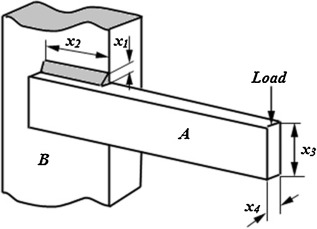
\includegraphics[scale=0.7]{Imgs/WB.jpg}
\end{center}
\captionsetup{justification=centering}
\caption{Schematic view of the welded beam design problem.}\label{fig:WB}
\end{figure}

We compare the results obtained by C-ITGO against a number of state of the art methods used to solve this problem, including PSO-DE, HPSO, MBA, CMA-ES, MVDE, CPSO, LCA, NM-PSO, APSO, WCA, IABC-MAL, IAPSO and SAMP-Jaya. Table \ref{tab:WB} shows the comparison of the statistical results obtained by all cited methods to solve the welded beam design problem. All the methods, with exception of CMA-ES, SAMP-Jaya and C-ITGO, took more than 10,000 iterations to achieve good quality solutions. C-ITGO achieved optimal solutions with a very small standard deviation of $3.65E \!-\! 12$ with ten times fewer function evaluations in average than most of the methods.


\begin{table*}[tp]
    \tiny
\begin{center}

\begin{tabular}{ P{2.0cm} P{2.0cm} P{2.0cm} P{2.0cm} P{2.0cm} P{2.0cm} P{2.0cm} P{2.0cm}  }
\hline
\textbf{Method} & \textbf{Best} & \textbf{Mean} & \textbf{Worst} & \textbf{SD} & \textbf{NFEs} \\
\hline
PSO-DE & 1.724852 & 1.724852 & 1.724852 & 6.70E-16 & 66,600 \\
HPSO & 1.724852 & 1.814295 & 1.749040 & 4.01E-02 & 81,000 \\
MBA & 1.724853 & 1.724853 & 1.724853 & 6.94E-19 & 47,340 \\
CPSO & 1.728024 & 1.748831 & 1.782143 & 1.29E-02 & 240,000 \\
LCA & 1.7248523 & 1.7248523 & 1.7248523 & 7.11E-15 & 15,000 \\
IABC-MAL & 1.724852 & 1.724852 & 1.724852 & 2.31E-12 & 15,000 \\
NM-PSO & 1.724717 & 1.726373 & 1.733393 & 3.50E-03 & 80,000 \\
IAPSO & 1.7248523 & 1.7248528 & 1.7248624 & 2.02E-06 & 12,500 \\
%Jaya & 1.724852 & 1.724852 & 1.724852 & 2.2E-08 & 4,739 \\
SAMP-Jaya & 1.724852 & 1.724852 & 1.724852 & 6.7E-16 & 3,618.25 \\
CI-TGO & 1.7248523 & 1.7248523 & 1.7248523 & 6.7E-16 & 1,166.84 \\


\hline
\end{tabular}
\end{center}

\caption{\fnt{8} Statistical results of different methods for Welded beam problem. \\[1em]}
\label{tab:WB}
\end{table*}



The results for C-ITGO and SAMP-Jaya are very similar, with same standard deviation, but with the former converging in less than one-third of the number of function evaluations. We note here that the best solution achieved by NM-PSO is slightly infeasible, so it should not be directly compared to the other methods.




\subsection{Tension / compression spring design problem}

This problem was introduced by \cite{TC}, and the objective is the minimization of the weight of a tension / compression spring (Figure \ref{fig:TC}). The problem has three continuous design variables, being them the diameter of spring wire, the diameter of spring mean coil and the number of active coils. It is subject to three nonlinear and one linear inequality constraints.

\begin{figure}[h]
\begin{center}
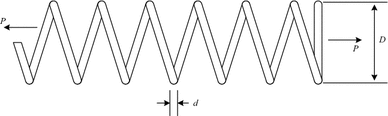
\includegraphics[scale=0.6]{Imgs/TC.png}
\end{center}
\captionsetup{justification=centering}
\caption{Schematic view of the tension/compression spring design problem}\label{fig:TC}
\end{figure}


A variety of methods were used in literature to solve the tension / compression spring design problem. Between them, we can cite HPSO, NM-PSO, MBA, PSO-DE, LCA, CB-ABC, QPSO, G-QPSO, APSO, CMA-ES, MVDE, DELC, IAPSO, IABC-MAL and SAMP-Jaya. Table \ref{tab:TC} shows the statistical results of all methods, along with the number of function evaluations taken to achieve such results.


\begin{table*}[tp]
    \tiny
\begin{center}

\begin{tabular}{ P{2.0cm} P{2.0cm} P{2.0cm} P{2.0cm} P{2.0cm} P{2.0cm} P{2.0cm} P{2.0cm}  }
\hline
\textbf{Method} & \textbf{Best} & \textbf{Mean} & \textbf{Worst} & \textbf{SD} & \textbf{MNFEs} \\
\hline

HPSO & 0.012665 & 0.012719 & 0.012707 & 1.58E-05 & 81,000 \\
NM-PSO & 0.012630 & 0.012633 & 0.012631 & 8.47E-07 & 80,000 \\
MBA & 0.012665 & 0.012713 & 0.012900 & 6.30E-05 & 7,650 \\
PSO-DE & 0.012665 & 0.012665 & 0.012665 & 1.20E-08 & 24,950 \\
LCA & 0.01266523 & 0.01266541 & 0.01266667 & 3.88E-07 & 15,000 \\
CB-ABC & 0.012665 & 0.012671 & N/A & 1.42E-05 & 15,000 \\
QPSO & 0.012669 & 0.018127 & 0.013854 & 1.34E-03 & 2,000 \\
G-QPSO & 0.012665 & 0.017759 & 0.013524 & 1.27E-03 & 2,000 \\
APSO & 0.012700 & 0.013297 & 0.014937 & 6.85E-04 & 120,000 \\
CMA-ES & 0.01266524 & 0.01266861 & 0.01269335 & 6.30E-06 & 19,445 \\
MVDE & 0.01266527 & 0.01266732 & 0.01271906 & 2.45E-06 & 10,000 \\
DELC & 0.012665 & 0.012666 & 0.012665 & 1.30E-07 & 20,000 \\
IAPSO & 0.01266523 & 0.013676527 & 0.01782864 & 1.573E-3 & 2,000 \\
IABC-MAL & 0.01266523 & 0.01266525 & 0.01266539 & 6.78E-08 & 15,000 \\
SAMP-Jaya & 0.012664 & 0.013193 & 0.012714 & 9.25E-05 & 6,861 \\
C-ITGO & 0.01266523 & 0.01266523 & 0.01266525 & 2.81E-9 & 535.08 \\

\hline
\end{tabular}
\end{center}

\caption{\fnt{8} Statistical results of different methods for tension/compression spring design problem. \\[1em]}
\label{tab:TC}
\end{table*}




The methods vary greatly in the number of function evaluations required to converge to good quality solutions. Only three of the methods (QPSO, G-QPSO and IAPSO) achieved convergence with 2,000 function evaluations, while some methods required more than 100,000. The best solution achieved by all methods have the same fitness value up to 3 decimal places.
 
The best solution reported by NM-PSO is again infeasible, so we do not compare it against other methods. The SAMP-Jaya method also seems to report a slightly infeasible best solution found, differing from the optimal value reported by other methods. However, the result differs only at the sixth decimal place, and the difference may be due to wrong rounding. We cannot state this for sure since we do not have access to the solution vector found by the method. Given the differences between the precision in the solutions reported by the methods, we consider $f(\bm{x}) = 0.012665$ to be the best solution found.

The C-ITGO method performed remarkably well on this problem, converging to the best solution found in 535.08 function evaluations on average, almost four times less than the second competing method. Also, the standard deviation is very small, in the order of $2.81E-9$. 

Given the relatively small domain of the problem, we believe that the C-ITGO method was able to cover the space efficiently, providing hot starting points for the local search method, which proved to be very effective in this case.




\subsection{Three-bar truss design problem}

The three-bar truss design problem \citep{TB} consists in minimizing the volume of a statically loaded three-bar truss. There are two continuous design variables and three nonlinear inequality constraints, based on the stress ($\sigma$) on each of the truss members. Figure \ref{fig:TB} shows the schematic view of the problem.

\begin{figure}[h]
\begin{center}
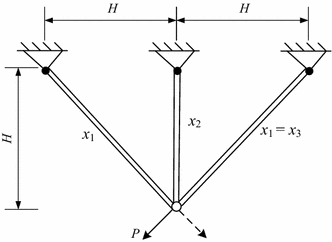
\includegraphics[scale=0.5]{Imgs/TB.png}
\end{center}
\captionsetup{justification=centering}
\caption{Schematic view of the three-bar truss design problem}\label{fig:TB}
\end{figure}


Here we present only the five best-performing methods used to solve this problem, since the solutions found in literature have very small variance from each other. These methods are CMA-ES, MVDE, DELC, MBA, and IABC-MAL. We present the statistical results for this problem in Table \ref{tab:TB}.


\begin{table*}[h]
    \tiny
\begin{center}

\begin{tabular}{ P{2.0cm} P{2.0cm} P{2.0cm} P{2.0cm} P{2.0cm} P{2.0cm} P{2.0cm} P{2.0cm}  }
\hline
\textbf{Method} & \textbf{Best} & \textbf{Mean} & \textbf{Worst} & \textbf{SD} & \textbf{MNFEs} \\
\hline

PSO-DE & 263.895843 & 263.895843 & 263.895843 & 4.50E-12 & 17,600 \\
CMA-ES & 263.895843 & 263.895843 & 263.895843 & 2.7E-09 & 1,706 \\
MVDE & 263.895843 & 263.895843 & 263.895855 & 2.58E-07 & 7,000 \\
DELC & 263.895843 & 263.895843 & 263.895843 & 4.3E-14 & 10,000 \\
MBA & 263.895852 & 263.897996 & 263.915983 & 3.93E-03 & 13,280 \\
IABC-MAL & 263.895843 & 263.895843 & 263.895843 & 0.0 & 15,000 \\
\textbf{C-ITGO} & \bf{263.895843} & \bf{263.895843} & \bf{263.895843} & \bf{2.0E-12} & \bf{136.48} \\


\hline
\end{tabular}
\end{center}
\vspace*{-6mm}
\caption{Statistical results of different methods for three-bar truss design problem. \\[1em]}
\label{tab:TB}
\end{table*}



From Table \ref{tab:TB} is possible to note that all methods have very similar results, differing mainly in the number of function calls. This is not surprising, given that the problem is simpler, has fewer variables and has a smaller domain than any other engineering design problem considered in this work.

C-ITGO achieved convergence quickly, taking 136.48 function evaluations in average. In this problem, we have set a small population, as well as a small number of function calls allowed in the local search procedure. Thus, we obtained the lowest NFEs than any of the competing techniques, at least ten times lower. It seems that the solutions found by the topographical heuristic were already close to the optimum, so the local search converged in very few iterations. However, the C-ITGO method has a slightly worse standard (less than 0.01\%) deviation than DELC and IABC-MAL.





\subsection{Speed reducer design problem}

In this problem, the total weight of the speed reducer (Figure \ref{fig:SR}) is to be minimized. The problem has seven design variables: face width, teeth module, number of teeth on the pinion, first and second length of shafts between bearings and first and second shafts diameter \citep{SR}. The problem has 11 nonlinear constraints, and the third variable is constrained to be an integer. We use two versions of this problem, where the only difference is in the bounds of the fifth variable. We will call this problems SRI and SRII, respectively.


\begin{figure}[h]
\begin{center}
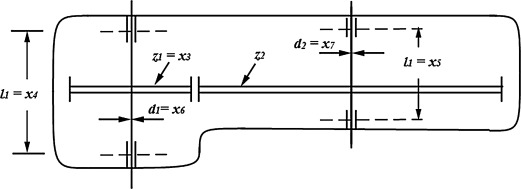
\includegraphics[scale=0.6]{Imgs/SR.jpg}
\end{center}
\captionsetup{justification=centering}
\caption{Schematic view of the speed reducer design problem}\label{fig:SR}
\end{figure}

For SRI, we compare C-ITGO results against 6 optimization methods, namely CPSO, LCA, IPSO, APSO, IAPSO and SAMP-Jaya, shown in Table \ref{tab:SP1}. The reported results for the SAMP-Jaya method seems to violate the integer constraint at variable three, but it is included so as to show that even in harder situations the C-ITGO algorithm can outperform any competing methods compared here.

The LCA, IPSO, IAPSO and C-ITGO present similar results, all finding the constrained global optimum solution and having very low standard deviation.

%The SiC-PSO and CPSO methods present inferior results, with higher average fitness. Besides having significant difference between the best from the mean fitness value, the SiC-PSO reports a standard deviation of 0.


\begin{table*}[tp]
    \tiny
    \begin{center}
    
    \begin{tabular}{ P{2.0cm} P{2.0cm} P{2.0cm} P{2.0cm} P{2.0cm} P{2.0cm} P{2.0cm} P{2.0cm}  }
    \hline
    \textbf{Method} & \textbf{Best} & \textbf{Mean} & \textbf{Worst} & \textbf{SD} & \textbf{MNFEs} \\
    \hline
    
    SiC-PSO & 2996.34816 & 2996.4085 & NA & 0.0 & 24,000 \\
    COPSO & 2996.372448 & 2996.408525 & NA & 2.867E-02 & 30,000 \\
    LCA & 2996.34816497 & 2996.34816497 & 2996.34816497 & 2.63E-12 & 24,000 \\
    IPSO & 2996.34816497 & 2996.3481 & 2996.34816509 & 2.43E-18 & 20,000 \\
    IAPSO & 2996.34816497 & 2996.34816497 & 2996.34816497 & 6,88E-13 & 6,000 \\
    CI-TGO & 2996.34816497 & 2996.34816497 & 2996.34816497 & 7.5E-13 & 856.40 \\
        
    \hline
    \end{tabular}
    \end{center}
    
    \caption{\fnt{8} Statistical results of different methods for the speed reducer design problem I. \\[1em]}
    \label{tab:SP1}
    \end{table*}
    
    

The first three methods take more than 20,000 iterations to converge to good quality solutions, while IAPSO and SAMP-Jaya take only 6,000 and 3744.66 NFEs respectively. C-ITGO outperforms the other methods by a large margin, converging in 858.40 function calls in average, while maintaining negligible higher standard deviation than IAPSO and IPSO.

For this problem, we used considerable greater populations, of sizes 150 and 10, while maintaining the number of allowed function evaluations of the local search relatively small (100 and 200). For the worst case, C-ITGO takes 3 full iterations to converge, while converging in the first iteration in most runs.

For SRII, the methods used for comparison were PSO-DE, MBA, WCA, DELC, CB-ABC, CMA-ES, MVDE, LCA, IABC-MAL, APSO, MBA, IPSO and IAPSO. From Table \ref{tab:SP2}, we can see that DELC, CMA-ES, MVDE, LCA, IAPSO and C-ITGO are the only methods that converged to the optimum in every run, having very small standard deviation. Although similar results are observed regarding the quality of the solutions, C-ITGO converges much faster than any competing method, using twelve times fewer function evaluations than IAPSO. The standard deviation achieved by C-ITGO is also the smallest among all compared methods.


\begin{table*}[h]
    \tiny
    \begin{center}
    
    \begin{tabular}{ P{2.0cm} P{2.0cm} P{2.0cm} P{2.0cm} P{2.0cm} P{2.0cm} P{2.0cm} P{2.0cm}  }
    \hline
    \textbf{Method} & \textbf{Best} & \textbf{Mean} & \textbf{Worst} & \textbf{SD} & \textbf{MNFEs} \\
    \hline
    
    PSO-DE & 2996.348167 & 2996.348174 & 2996.348204 & 6.40E-06 & 54,350 \\
    WCA & 2994.471066 & 2994.474392 & 2994.505578 & 7.4E-03 & 15,150 \\    
    DELC & 2994.471066 & 2994.471066 & 2994.471066 & 1.90E-12 & 30,000 \\
    CB-ABC & 2994.471066 & 2994.471066 & N/A & 2.48E-07 & 15,000 \\
    CMA-ES & 2994.471066 & 2994.471066 & 2994.471066 & 8.98E-10 & 12,998 \\
    MVDE & 2994.471066 & 2994.471066 & 2994.471066 & 2.82E-07 & 30,000 \\    
    IABC-MAL & 2994.471066 & 2994.471066 & 2994.471066 & 8.51E-13 & 15,000 \\ 
    LCA & 2994.471066 & 2994.471066 & 2994.471066 & 2.66E-12 & 24000 \\
    APSO & 3187.630486 & 3822.640624 & 4443.017639 & 366.146 & 30,000 \\
    MBA & 2994.482453 & 2996.769019 & 2999.652444 & 1.56 & 6300 \\
    IPSO & 2994.471067 & 2994.47108 & 2994.4711 & 9.27E-06 & 20,000 \\
    IAPSO & 2994.471066 & 2994.471066 & 2994.471066 & 2.65E-09 & 6,000 \\
    SAMP-Jaya & 2760.673988 & 2760.673988 & 2760.673988 & 2.54E-11 & 3744.66 \\    
    \textbf{C-ITGO} & \bf{2994.471066} & \bf{2994.471066} & \bf{2994.471066} & \bf{9.28E-13} & \bf{491.24} \\ 
    
  

    \hline
    \end{tabular}
    \end{center}
    \vspace*{-6mm}
    \caption{Statistical results of different methods for the speed reducer design problem II. \\[1em]}
    \label{tab:SP2}
    \end{table*}
    
    

For this specific problem, we used the SQP algorithm as local search, and rounded the value of the third variable. In this case, this approach proved to converge much faster than using a mixed integer local search. Also, the first population size is considerable smaller than the one used in SRI (100 in this problem).



\subsection{Pressure vessel design problem}

In the pressure vessel design problem, the objective is to minimize the total manufacturing cost, including the cost of the material, forming and welding costs \citep{PV}. The problem is subject to three linear and one nonlinear inequality constraint, and its structure is shown in Figure \ref{fig:PV}. The four variables are the thickness of the shell, the thickness of the head, the inner radius, and the length of the cylindrical section of the vessel. This is an example of a mixed integer problem, where the first and second variables are constrained to be integers.


\begin{figure}[h]
\begin{center}
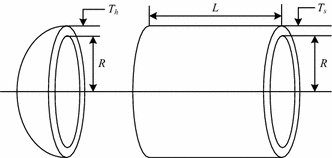
\includegraphics[scale=0.6]{Imgs/PV.png}
\end{center}
\captionsetup{justification=centering}
\caption{Schematic view of pressure vessel design problem.}\label{fig:PV}
\end{figure}


%Some methods in literature optimized the pressure vessel design problem without taking into account the integer constraints at the first and second variables. So, to compare the C-ITGO performance, we will only consider methods that respect the integer constraints.


\begin{table*}[h]
    \tiny
    \begin{center}
    
    \begin{tabular}{ P{2.0cm} P{2.0cm} P{2.0cm} P{2.0cm} P{2.0cm} P{2.0cm} P{2.0cm} P{2.0cm}  }
    \hline
    \textbf{Method} & \textbf{Best} & \textbf{Mean} & \textbf{Worst} & \textbf{SD} & \textbf{MNFEs} \\
    \hline
    
    UPSO & 6544.2700 & 9032.5500 & N/A & 9.95E+02 & 100,000 \\
    QPSO & 6059.7209 & 8017.2816 & 6440.3786 & 4.79E+02 & 8,000 \\
    G-QPSO & 6059.7208 & 7544.4925 & 6440.3786 & 4.48E+02 & 8,000 \\
    CMA-ES & 6059.7143 & 6170.25055 & 6410.08676 & 140.4843 & 30,018 \\
    MVDE & 6059.7144 & 6059.99724 & 6090.53353 & 2.9103 & 15,000 \\ 
    CB-ABC & 6059.7143 & 6126.6237 & N/A & 1.14E+02 & 15,000 \\
    PSO-DE & 6059.7140 & 6059.7140 & N/A & N/A & 42,100 \\
    HPSO & 6059.7143 & 6099.9323 & 6288.6770 & 86.2000 & 81,000 \\
    WCA & 5885.3327 & 6198.6172 & 6590.2129 & 213.0490 & 27,500 \\
    LCA & 6059.8553 & 6070.5884 & 6090.6114 & 11.37534 & 24,000 \\
    APSO & 6059.7242 & 6470.7156 & 7544.4927 & 326.9688 & 200,000 \\
    CPSO & 6061.0777 & 6147.1332 & 6363.8041 & 86.4500 & 240,000 \\
    MBA & 5889.3216 & 6200.64765 & 6392.5062 & 160.34 & 70,650 \\    
    IPSO & 6059.7143 & 6059.7155 & 6059.7257 & 0.00232 & 20,000 \\
    DELC & 6059.7143 & 6059.7143 & 6059.7143 & 2.10E-11 & 30,000 \\  
    IABC-MAL & 6059.7143 & 6072.5972 & 6089.2720 & 1.88E-06 & 15,000 \\
    SAMP-Jaya & 5872.2129 & 5872.2129 & 5872.2129 & 5.0E-12 & 6513.33 \\    
    IAPSO & 6059.7143 & 6068.7539 & 6090.5314 & 14.0057 & 7,500 \\
    \textbf{C-ITGO} & \bf{6059.7143} & \bf{6059.7143} & \bf{6059.7143} & \bf{9.8E-13} & \bf{1101.64} \\
    
    \hline
    \end{tabular}
    \end{center}
    \vspace*{-6mm}
    \caption{Statistical results of different methods for the pressure vessel design problem. \\[1em]}
    \label{tab:PV}
    \end{table*}
    
    

We compare C-ITGO against the  QPSO, G-QPSO, CMA-ES, MVDE, CB-ABC, HPSO, WCA, LCA, APSO, MBA, IABC-MAL, SAMP-Jaya and IAPSO methods. The statistical results are shown in Table \ref{tab:PV}. Some of the methods used to solve this problem report unfeasible results (WCA, MBA and SAMP-Jaya), probably because the integer constraints are ignored. Nevertheless, we still use the results of these methods to prove the superior convergence of C-ITGO, even in constrained mixed integer problems.


The algorithms CMA-ES, CB-ABC, HPSO, IABC-MAl, IAPSO and C-ITGO are the only who found the feasible optimal solution. All other methods presented relatively poor performance, with much higher NFEs in average. C-ITGO takes less than five times the number of function evaluations to converge than the best competing method, SAMP-Jaya, which reported a result of 6,513.33 NFEs. Also, C-ITGO achieves the smallest standard deviation among all methods. All runs of C-ITGO converged quickly to the global optimum, showing unarguably better results than any other method used for comparison for this problem.



\subsection{Gear train design problem}

In this problem, the objective is to minimize the cost of the gear ratio of the gear train \citep{PV}. An example is shown in Figure \ref{fig:GT}. The problem has four variables, representing the number of teeth for the four gears. The only constraint of the problem is that all variables must be integers.


\begin{figure}[h]
\begin{center}
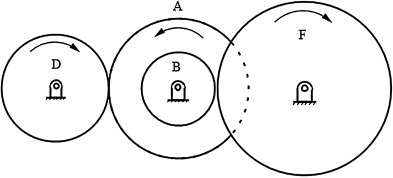
\includegraphics[scale=0.6]{Imgs/GT.jpg}
\end{center}
\captionsetup{justification=centering}
\caption{Gear train design problem structure.}\label{fig:GT}
\end{figure}


We compare the C-ITGO results, shown in Table \ref{fig:GT}, against other five methods: MBA, UPSO, CS, APSO and IAPSO. In general, all methods compared achieved similar results, having found the optimal solution for the problem. UPSO failed at finding some solutions, while APSO has a considerable greater mean value than other the methods.
The main difference relies on the number of function calls, varying from 100,00 for UPSO to 800 for IAPSO.


\begin{table*}[tp]
    \tiny
\begin{center}

\begin{tabular}{ P{2.0cm} P{2.0cm} P{2.0cm} P{2.0cm} P{2.0cm} P{2.0cm} P{2.0cm} P{2.0cm}  }
\hline
\textbf{Method} & \textbf{Best} & \textbf{Mean} & \textbf{Worst} & \textbf{SD} & \textbf{MNFEs} \\
\hline

MBA & 2.700857E-12 & 2.062904E-08 & 2.47E-09 & 3.94E-09 & 1120 \\
UPSO & 2.700857E-12 & 3.80562E-08 & N/A & 1.09E-07 & 100,000 \\
CS & 2.7009E-12 & 1.9841E-9 & 2.3576E-9 & 3.55E-9 & 5,000 \\
APSO & 2.700857E-12 & 4.781676E-07 & 7.072678E-06 & 1.44E-06 & 8,000 \\
IAPSO & 2.700857E-12 & 5.492477E-09 & 1.827380E-08 & 6.36E-09 & 800 \\
C-ITGO & 2.700857E-12 & 4.6504232E-09 & 2.7264505E-08 & 6.85E-09 & 773.0 \\


\hline
\end{tabular}
\end{center}
\vspace*{-6mm}
\caption{Statistical results of different methods for the gear train design problem. \\[1em]}
\label{tab:GT}
\end{table*}




Since this is an integer optimization problem, we used the mixed integer local search based on the NOMAD solver. In this problem, the solver had some difficulty in some runs, achieving $6.85E \! - \! 09$ of standard deviation, more than IAPSO, CS and MBA. The mean fitness value, however, is just worse than the CS method, which takes 5,000 function calls to converge. Besides this drawbacks, C-ITGO converges faster than the other methods compared here, taking only 773.0 function calls on average.



\subsection{Multiple disk clutch brake design problem}

This is also an example of a problem where all variables are discrete. The Multiple disk clutch brake design problem aims at minimizing the mass of a multiple disc clutch brake \cite{MD}. There are five integer variables: the inner radius, outer radius, thickness of the disc, actuating force and number of friction surfaces (Figure \ref{fig:MD}). The problem is also constrained by nine nonlinear inequalities.

\begin{figure}[h]
\begin{center}
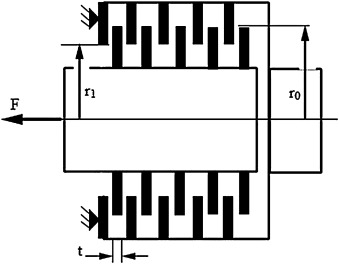
\includegraphics[scale=0.6]{Imgs/MD.jpg}
\end{center}
\captionsetup{justification=centering}
\caption{Schematic view of the multiple disk clutch brake design problem.}\label{fig:MD}
\end{figure}

To compare the results, we used only methods who achieved close performance to the obtained by C-ITGO, since some methods in literature have very diverging results. The WCA, IPSO, APSO and IAPSO methods achieved good performance in this problem, finding the optimal solution and having very small variance, as shown in Table \ref{tab:MD}. The WCA and IAPSO took very few function evaluations to converge, respectively 500 and 400. IPSO took long more, with 20,000 function evaluations. However, the reported standard deviation for IPSO was 0.0.


\begin{table*}[tp]
    \tiny
    \begin{center}
    
    \begin{tabular}{ P{2.0cm} P{2.0cm} P{2.0cm} P{2.0cm} P{2.0cm} P{2.0cm} P{2.0cm} P{2.0cm}  }
    \hline
    \textbf{Method} & \textbf{Best} & \textbf{Mean} & \textbf{Worst} & \textbf{SD} & \textbf{NFEs} \\
    \hline

    WCA & 0.313656 & 0.313656 & 0.313656 & 1.69E-16 & 500 \\
    IPSO & 0.313656 & 0.313656 & 0.313656 & 0.0 & 20,000 \\
    IAPSO & 0.313656 & 0.313656 & 0.313656 & 1.13E-16 & 400 \\
    CI-TGO & 0.313656 & 0.313656 & 0.313656 & 1.13E-16 & 286.48 \\

    \hline
    \end{tabular}
    \end{center}
    
    \caption{\fnt{8} Statistical results of different methods for the multiple disk clutch break design problem. \\[1em]}
    \label{tab:MD}
    \end{table*}
    
    

The C-ITGO clearly outperforms the other methods, having a standard deviation of $1.13E-16$, while converging with only 286.48 function evaluations on average. For this problem, we also have used a very small populations of size 20 and 5. The number of function evaluations in the first step was 100, and most runs converged in much less, enjoying the quality of initial solutions provided by the topographical heuristic step. Some runs, however, took more than 1,500 function evaluations, bringing the mean NFEs up.



\subsection{Best Solutions}

Table \ref{tab:BestResults} shows the fitness value, the values of the variables and the values of the constraints for the best solution found by C-ITGO for all problems. The precision for the results of each problem was set to match the results reported by the competing methods cited in this work. However, to the best of our knowledge, the best solution found by C-ITGO for each problem is equal to, or negligibly worse (up to several decimal places) than the best solutions reported by state of the art methods.


\noindent
\begin{table*}[tp]
    \tiny
\begin{center}
\begin{adjustwidth}{-1cm}{}
\begin{tabular}{ | P{1.0cm} | P{1.5cm} |  P{1.5cm} | P{1.5cm} | P{1.5cm} | P{1.5cm} | P{1.5cm} | P{1.5cm} | P{1.5cm} |  }
\hline
\textbf{Prob.} & \textbf{WB} & \textbf{TC} & \textbf{TB} & \textbf{SRI} & \textbf{SRII} & \textbf{PV} & \textbf{GT} & \textbf{MD} \\
\hline
\rule{0pt}{3ex}
$f(\cdot)$ & 1.7248523 & 0.01266523 & 263.895843 & 2996.34816497 & 2994.471066 & 6059.7143 & 2.700857E-12 & 0.313656 \\
\hline
\rule{0pt}{3ex}
$\bm{x}_1$ &  0.2057296 & 0.05168906 & 0.788675 & 3.5 & 3.5 & 13.0 & 43 & 70  \\
$\bm{x}_2$ &  3.4704886 & 0.35671774 & 0.408248 & 7.0 & 0.7 & 7.0 & 16 & 90 \\
$\bm{x}_3$ &  9.0366239 & 11.28896574 & & 17 & 17 & 41.5984 & 19 &  1  \\
$\bm{x}_4$ &  0.2057296 & & & 7.3 & 7.3 & 176.6366 & 49 & 830  \\
$\bm{x}_5$ & & & & 7.8 & 7.715320 & & & 3 \\
$\bm{x}_6$ & & & & 3.35021467 & 3.350215 & & &   \\
$\bm{x}_7$ & & & & 5.28668323 & 5.286654 & & &   \\
\hline
\rule{0pt}{3ex}
$\bm{g}_1$ & 0.0 & 0.0 & 0.0 & -0.07391528 & -0.073915 & -2.6645E-15 & & 0.0  \\
$\bm{g}_2$ & 0.0 & 0.0 & -1.464102 & -0.19799853 & -0.197999 & -0.0359 & & -24.0  \\
$\bm{g}_3$ & 0.0 & -4.05378563 & -0.535898 & -0.49917225 & -0.499172 & -4.4238E-09 & & -0.917438 \\
$\bm{g}_4$ & -3.4329838 & -1.09159320 & & -0.90147170 & -0.904644 & -63.3634 & & -9.826183  \\
$\bm{g}_5$ & -0.0807296 & & & -8.846257E-13 & -2.220446E-16 & & &  -7.894697 \\
$\bm{g}_6$ & -0.2355403 & & & -4.885758E-12 & 0.0 & & & -0.173855  \\
$\bm{g}_7$ & -1.818989E-12 & & & -0.7025 & -0.7025 & & & -40.118750 \\
$\bm{g}_8$ & & & & -1.887379E-15 & 0.0 & & &  -14.826145 \\
$\bm{g}_9$ & & & & -0.58333333 & -0.583333 & & &    \\
$\bm{g}_{10}$ & & & & -0.05132575 & -0.051326 & & &    \\
$\bm{g}_{11}$ & & & & -0.01085237 & 0.0 & & &    \\
\hline
\end{tabular}
\end{adjustwidth}
\end{center}
\vspace*{-6mm}
\caption{Results for the best solution found by C-ITGO for each engineering design problem.. \\[1em]}
\label{tab:BestResults}
\end{table*}








\iffalse

\begin{align*}
\textbf{Minimize:} & \\
& f(\bm{x}) = 1.10471x_1^2x_2 + 0.04811x_3x_4(14 + x_2) \\[0.5em]
\textbf{subject to:} & \\
& g_1(\bm{x}) = \tau(\bm{x}) - 13,600 \leq 0 \\
& g_2(\bm{x}) = \sigma(\bm{x}) - 30,000 \leq 0 \\
& g_3(\bm{x}) = x_1 - x_4 \leq 0 \\
& g_4(\bm{x}) = 0.10471x_1^2 + 0.04811x_3x_4(14+x_2) - 5  \leq 0 \\
& g_5(\bm{x}) = 0.125 - x_1 \leq 0 \\
& g_6(\bm{x}) = \delta(\bm{x}) - 0.25 \leq 0 \\
& g_7(\bm{x}) = 6,000 - Pc(\bm{x}) \leq 0 \\[0.5em]
\textbf{where:} & \\
& \tau(\bm{x}) = \sqrt{\tau^2 + \frac{(2 \tau' \tau'' x_2)}{2R} + \tau''^2 } \\
& \tau' = \frac{6,000}{(sqrt{2} x_1 x_2)} \\[0.5em]
& \tau'' = \frac{(M R)}{J} \\
& M = 6,000 (14 + \frac{x_2}{2}) \\
& R = sqrt{\frac{x_2^2}{4} + (x_1 + \frac{x_3}{2})^2} \\
& J = 2 x_1 x_2 \sqrt{2} (\frac{x_2^2}{12} + (x_1 + \frac{x_3}{2})^2) \\[0.5em]
& \sigma(\bm{x}) = 504,000 / (x_4 x_3^2) \\
& \delta(\bm{x}) = \frac{65,856,000}{(30 \times 10^6 x_4 x_3^3)} \\
& Pc(\bm{x}) = \frac{4.013(30 \times 10^6)}{196} \sqrt{x_3^2 \frac{x_4^6}{36}} \Bigg(1 - \frac{x_3}{28} \sqrt{\frac{30 \times 10^6}{4(12 \times 10^6)}}\Bigg) \\[0.5em]
\textbf{with bounds:} & \\
&  0.1 \leq x_1, x_4 \leq 2 \\
&  0.1 \leq x_2, x_3 \leq 10
\end{align*}

\begin{equation*}
\begin{aligned}
%& \textbf{Minimize:} \\
& f(\bm{x}) = 0.6224z_1x_3x_4 + 1.7781z_2x_3^2 + 3.1661z_1^2x_4 + 19.84z_1^2x_3 \\[0.5em]
& \textbf{subject to:}\\
& g_1(\bm{x}) = -z_1 + 0.193x_3 \leq 0 \\
& g_2(\bm{x}) = -z_2 + 0.00954x_3 \leq 0 \\
& g_3(\bm{x}) = -\pi x_3^2x_4^2 - \frac{4}{3} \pi x_3^3 + 1,296,000 \leq 0 \\
& g_4(\bm{x}) = x_4 - 240  \leq 0 \\[0.5em]
& \textbf{where:} \\
& z_1 = 0.0625x_1 \\
& z_2 = 0.0625x_2 \\[0.5em]
& \textbf{with bounds:} \\
& 1 \leq x_1, x_2 \leq 99 \\
& 10 \leq x_2, x_3 \leq 200 \\
& x_1, x_2 \in \mathbb{Z}
\end{aligned}
\end{equation*}

\begin{equation*}
\begin{aligned}
%& \textbf{Minimize:} \\
& f(\bm{x}) = 0.7854x_1x_2^2(3.333x_3^2 + 14.9334x_3 - 43.0934) \\
& \quad \qquad - 1.508x_1(x_6^2 + x_7^2) + 7.4777(x_6^3 + x_7^3) \\
& \quad \qquad + 0.7854(x_4 x_6^2 + x_5x_7^2) \\[0.5em]
& \textbf{subject to:}\\
& g_1(\bm{x}) = \frac{27}{x_1x_2^2x_3} - 1 \leq 0 \\
& g_2(\bm{x}) = \frac{397.5}{x_1x_2x_3^2} - 1 \leq 0 \\
& g_3(\bm{x}) = \frac{1.93x_4^3}{x_2x_3x_6^4} -1 \leq 0 \\
& g_4(\bm{x}) = \frac{1.93x_5^3}{x_2x_3x_7^4} -1 \leq 0 \\
& g_5(\bm{x}) = \frac{1}{110x_6^3} \sqrt{\Big( \frac{745x_4}{x_2x_3} \Big)^2 + 16.9 \times 10^6} - 1 \leq 0 \\
& g_6(\bm{x}) = \frac{1}{85x_7^3} \sqrt{\Big( \frac{745x_5}{x_2x_3} \Big)^2 + 157.5 \times 10^6} - 1 \leq 0 \\
& g_7(\bm{x}) = \frac{x_2x_3}{40} - 1 \leq 0 \\
& g_8(\bm{x}) = \frac{5x_2}{x_1} - 1 \leq 0 \\
& g_9(\bm{x}) = \frac{x_1}{12x_2} - 1 \leq 0 \\
& g_{10}(\bm{x}) = \frac{1.5x_6 + 1.9}{x_4} - 1 \leq 0 \\
& g_{11}(\bm{x}) = \frac{1.1x_7 + 1.9}{x_5} - 1 \leq 0 \\[0.5em]
& \textbf{with bounds:} \\
& 2.6 \leq x_1 \leq 3.6, \quad 0.7 \leq x_2 \leq 0.8, \quad 17 \leq x_3 \leq 28, \quad 7.3 \leq x_4 \leq 8.3 \\
& 7.8 \leq x_5 \leq 8.3, \quad 2.9 \leq x_6 \leq 3.9, \quad 5.0 \leq x_7 \leq 5.5
\end{aligned}
\end{equation*}

\begin{equation*}
\begin{aligned}
%& \textbf{Minimize:} \\
& f(\bm{x}) = (x_3 + 2)x_2x_1^2 \\[0.5em]
& \textbf{subject to:}\\
& g_1(\bm{x}) = 1 - \frac{x_2^3 x_3}{7.1785 x_1^4} \leq 0 \\
& g_2(\bm{x}) = \frac{4x_2^2 - x_1 x_2}{12,566 (x_2 x_1^3) - x_1^4} + \frac{1}{5.108 x_1^2} - 1 \leq 0 \\
& g_3(\bm{x}) = 1 - \frac{140.45 x_1}{x_2^2 x_3} \leq 0 \\
& g_4(\bm{x}) = \frac{x_2 + x_1}{1.5} - 1 \leq 0 \\[0.5em]
& \textbf{with bounds:} \\
& 0.05 \leq x_1 \leq 2, \quad 0.25 \leq x_2 \leq 1.3, \quad 2 \leq x_3 \leq 15
\end{aligned}
\end{equation*}

\begin{equation*}
\begin{aligned}
%& \textbf{Minimize:} \\
& f(\bm{x}) = \Big(\Big(\frac{1}{6.931}\Big) - \Big(\frac{x_2 x_3}{x_1 x_4} \Big)  \Big)^2 \\[0.5em]
& \textbf{with bounds:} \\
& 12 \leq x_i \leq 60, \quad i = 1, 2, 3, 4 \\
& x_i \in \mathbb{Z}, \quad i = 1, 2, 3, 4
\end{aligned}
\end{equation*}

\begin{equation*}
\begin{aligned}
%\textbf{Minimize:} & \\
& f(\bm{x}) = \pi(x_2^2 - x_1^2) x_3 (x_5 + 1) \rho \\[0.5em]
& \textbf{subject to:} \\
& g_1(\bm{x}) = x_2 - x_1 - \Delta R \geq 0 \\
& g_2(\bm{x}) = L_{max} - (x_5 + 1) (x_3 + \delta) \geq 0 \\
& g_3(\bm{x}) = p_{max} - p_{rz} \geq 0 \\
& g_4(\bm{x}) = p_max * Vsr_{max} - p_{rz} * Vsr \geq 0 \\
& g_5(\bm{x}) = Vsr_{max} - Vsr \geq 0 \\
& g_6(\bm{x}) = T_{max} - T \geq 0 \\
& g_7(\bm{x}) = M_h - s  M_s \geq 0 \\
& g_7(\bm{x}) = T \geq 0 \\[0.5em]
& \textbf{where:} \\
& M_h = \frac{2}{3} \mu x_4 x_5 \frac{x_2^3 - x_1^3}{x_2^2 - x_1^2} N \cdot mm  \\
& \omega = \frac{\pi n}{30} rad/s  \\
& A = \pi (x_2^2 - x_1^2) mm^2  \\
& p_{rz} = \frac{x_4}{A} N/mm^2 \\
& V_{sr} = \frac{pi R_{sr} n}{30} mm /s \\
& R_{sr} = \frac{2}{3} \frac{x_2^3 - x_1^3}{x_2^2 x_1^2} mm \\
& \Delta R = 20mm, \quad L_{max} = 30mm, \quad \mu = 0.6 \\
& p_{max} = 1MPa, \quad \rho = 0.0000078kg/mm^3 \\
& Vsr_{max} = 10m/s, \quad \delta = 0.5mm, \quad s = 1.5; \\
& T_{max} = 15s, \quad n = 250rpm, \quad I_{z} = 55Kg \cdot m^2 \\
& M_s = 40Nm, \quad Mf = 3Nm \\[0.5em]
& \textbf{with bounds:} \\
& 60 \leq x_1 \leq 80, \quad 90 \leq x_2 \leq 110, \quad 1 \leq x_3 \leq 3 \\
& 0 \leq x_4 \leq 1000, \quad 2 \leq x_5 \leq 9
\end{aligned}
\end{equation*}

\begin{equation*}
\begin{aligned}
%& \textbf{Minimize:} \\
& f(\bm{x}) = 2 \sqrt{2} x_1 + x_2 * l \\[0.5em]
& \textbf{subject to:}\\
& g_1(\bm{x}) = \frac{\sqrt{2} x_1 + x_2}{\sqrt{2} x_1^2 + 2 x_1 x_2} P - \sigma \leq 0 \\
& g_2(\bm{x}) = \frac{x_2}{\sqrt{2} x_1^2 + 2 x_1 x_2} P - \sigma \leq 0 \\
& g_3(\bm{x}) = \frac{1}{\sqrt{2} x_2 + x_1 x_2} P - \sigma \leq 0 \\[0.5em]
& \textbf{where:} \\
& l = 100cm, \quad P = 2 kN/cm^2, \quad \sigma = 2 kN/cm^2 \\[0.5em]
& \textbf{with bounds:} \\
& 0 \leq x_1, x_2 \leq 1
\end{aligned}
\end{equation*}

\fi
